\index{backpropagation}
We now derive the gradient.  The derivation is short once the notation of
Section~\ref{sec:nnnotation} is in place, but the indices hide what is going
on, so we first work through the two smallest networks there are: a single
neuron with a scalar input and a scalar output, which is the logistic
regression of Figure~\ref{fig:5-neuron} with a different loss, and the same
neuron with one hidden neuron in front of it.  Everything that
Section~\ref{sec:backpropgeneral} does with matrices and sums, these two
examples do with products of scalars, and the second of them already contains
the backpropagation equation.

%......................................................................
\subsection{Two scalar examples: no hidden layer and one hidden layer}
\label{sec:backpropscalar}

\index{backpropagation!scalar example}\index{delta rule}
Throughout this subsection every layer has one node, so the node indices $i,j$
of Eq.~(\ref{eq:8-zdef}) are dropped and only the layer superscript remains:
$w^{l}$, $b^{l}$, $z^{l}$ and $a^{l}$ are numbers, not arrays.  We take the
sigmoid $\sigma$ of Eq.~(\ref{eq:8-sigmoid}) as activation, with
$\sigma'(z)=\sigma(z)(1-\sigma(z))$, and the half-squared error of
Eq.~(\ref{eq:8-mse}) for a single training pair $(x,y)$.  Nothing depends on
these choices; for another activation replace $\sigma'$ by $f'$, and for
another loss replace $a^{L}-y$ by $\partial C/\partial a^{L}$.

\paragraph{No hidden layer.}
The network is one neuron,
\begin{equation}
  x \;\longrightarrow\; z^{1}=w^{1}x+b^{1}
    \;\longrightarrow\; a^{1}=\sigma\!\left(z^{1}\right)
    \;\longrightarrow\; C=\tfrac12\left(a^{1}-y\right)^{2},
  \label{eq:8-scalarone}
\end{equation}
with the two trainable parameters $\bm{\Theta}=\{w^{1},b^{1}\}$.  It is the
neuron of Figure~\ref{fig:5-neuron} with $p=1$ input and the cross entropy
replaced by the squared error, and the top panel of
Figure~\ref{fig:8-scalargraph} draws it.  Training means moving $w^{1}$ and
$b^{1}$ so as to reduce the discrepancy between the prediction $a^{1}$ and the
target $y$, and for that we need $\partial C/\partial w^{1}$ and
$\partial C/\partial b^{1}$.  The cost depends on $w^{1}$ only along the path
$w^{1}\to z^{1}\to a^{1}\to C$, so the chain rule~(\ref{eq:1-chainrule}) gives
\begin{equation}
  \frac{\partial C}{\partial w^{1}}
   = \frac{\partial C}{\partial a^{1}}
     \frac{\partial a^{1}}{\partial z^{1}}
     \frac{\partial z^{1}}{\partial w^{1}}
   = \left(a^{1}-y\right)\sigma'\!\left(z^{1}\right)x ,
  \label{eq:8-scalaronew}
\end{equation}
and the same path with $\partial z^{1}/\partial b^{1}=1$ as its last factor
gives $\partial C/\partial b^{1}=(a^{1}-y)\sigma'(z^{1})$.  The two gradients
share everything except the last factor, and it pays to give the shared part
a name.  Define the \emph{error} of the neuron,
\begin{equation}
  \delta^{1} = \left(a^{1}-y\right)\sigma'\!\left(z^{1}\right)
             = \frac{\partial C}{\partial z^{1}} ,
  \label{eq:8-scalardelta}
\end{equation}
the sensitivity of the cost to the pre-activation.  Then
\begin{equation}
  \frac{\partial C}{\partial w^{1}} = \delta^{1}x,
  \qquad
  \frac{\partial C}{\partial b^{1}} = \delta^{1},
  \label{eq:8-scalargrad}
\end{equation}
and one step of gradient descent with learning rate $\gamma$ reads
\begin{equation}
  w^{1}\leftarrow w^{1}-\gamma\,\delta^{1}x ,
  \qquad
  b^{1}\leftarrow b^{1}-\gamma\,\delta^{1} .
  \label{eq:8-scalarupdate}
\end{equation}
Each update is an error term, $\delta^{1}$, multiplied by the signal that
entered the parameter: $x$ for the weight and the constant $1$ for the bias.
This is the delta rule of Eq.~(\ref{eq:5-deltarule}) once more, with one
difference that is worth pausing on.  For logistic regression the derivative
of the cross entropy with respect to $z$ was the bare residual $\hat p-y$,
Eq.~(\ref{eq:5-gradone}), because the derivative of the softplus cancelled
the derivative of the sigmoid.  With the squared error nothing cancels and the
residual is multiplied by $\sigma'(z^{1})$, which is at most $1/4$ and
decays to zero as soon as $|z^{1}|$ is a few units.  A saturated neuron
therefore learns slowly however wrong it is; this is the factor $f'$ that
Section~\ref{sec:backpropgeneral} will find in front of every error, and the
seed of the vanishing gradients of Section~\ref{sec:vanishing}.

\paragraph{The same neuron, read backwards.}
\index{automatic differentiation!and backpropagation}
Section~\ref{sec:logregad} computed the gradient of logistic regression by
writing the neuron as an evaluation trace and sweeping it in reverse.  The
same can be done here, and the result identifies $\delta^{1}$.  With the
parameters as inputs, $v_{-1}=b^{1}$ and $v_{0}=w^{1}$, and the data as
constants, the trace of Eq.~(\ref{eq:8-scalarone}) is
\begin{equation}
  v_{1}=v_{0}\,x,\qquad
  v_{2}=v_{1}+v_{-1}=z^{1},\qquad
  v_{3}=\sigma(v_{2})=a^{1},\qquad
  v_{4}=\tfrac12\left(v_{3}-y\right)^{2}=C .
  \label{eq:8-scalartrace}
\end{equation}
The reverse sweep of Eq.~(\ref{eq:4-reverserec}) starts from $\bar v_{4}=1$
and multiplies by the local derivatives on the way back:
\begin{equation}
  \bar v_{3}=\bar v_{4}\left(v_{3}-y\right)=a^{1}-y,\qquad
  \bar v_{2}=\bar v_{3}\,\sigma'(v_{2})=\delta^{1},\qquad
  \bar v_{0}=\bar v_{2}\,x=\delta^{1}x,\qquad
  \bar v_{-1}=\bar v_{2}=\delta^{1} .
  \label{eq:8-scalarreverse}
\end{equation}
The error $\delta^{1}$ is the \emph{adjoint of the pre-activation}, exactly as
$\bar z=\hat p-y$ was in Figure~\ref{fig:5-neuron}, and
Eq.~(\ref{eq:8-scalargrad}) is what the sweep delivers when it reaches the two
inputs.  One sweep gives both gradients; the forward mode of
Eq.~(\ref{eq:4-forwardrec}) would need one sweep per parameter, the same
comparison as in Section~\ref{sec:logregad}.  Backpropagation, we shall see,
is this sweep continued through as many layers as the network has.

\begin{figure}[htbp]
\centering
\begin{tikzpicture}[>=Latex,x=1cm,y=1cm,
  inp/.style={circle,draw=black!65,fill=Blue3!12,minimum size=8mm,
              inner sep=0pt,font=\small},
  bia/.style={circle,draw=black!65,fill=Red3!12,minimum size=7mm,
              inner sep=0pt,font=\small},
  nr/.style={circle,draw=black!65,fill=orange!18,minimum size=15mm,
             inner sep=1pt,font=\footnotesize,align=center},
  ls/.style={rectangle,rounded corners=1pt,draw=black!65,dashed,fill=black!3,
             minimum height=9mm,minimum width=14mm,inner sep=2pt,font=\small},
  wl/.style={font=\footnotesize,fill=white,inner sep=1pt},
  bk/.style={font=\footnotesize,Red3},
  rv/.style={->,Red3,dashed}]
  % ---- top: no hidden layer ----
  \node[font=\footnotesize,black!60,anchor=west] at (-1.0,2.75)
       {no hidden layer, Eq.~(\ref{eq:8-scalarone})};
  \node[inp] (x) at (0,0.8) {$x$};
  \node[bia] (b1) at (2.6,-0.9) {$1$};
  \node[nr]  (n1) at (2.6,0.8) {$z^{1}$\\$\downarrow$\\$a^{1}$};
  \node[ls]  (C) at (6.2,0.8) {$\tfrac12(a^{1}-y)^{2}$};
  \node[inp] (y) at (6.2,-0.9) {$y$};
  \draw[->,black!70] (x) -- node[wl,pos=0.45]{$w^{1}$} (n1);
  \draw[->,black!70] (b1) -- node[wl,pos=0.5]{$b^{1}$} (n1);
  \draw[->,black!70] (n1) -- node[above,font=\footnotesize]{$a^{1}$} (C);
  \draw[->,black!70] (y) -- (C);
  \draw[->,black!70] (C) -- ++(1.4,0) node[right,font=\small] {$C$};
  \draw[rv] (5.2,0.35) -- (3.6,0.35);
  \node[bk] at (4.4,0.05) {$\bar a^{1}=a^{1}-y$};
  \node[bk] at (2.6,1.95) {$\delta^{1}=\bar z^{1}=(a^{1}-y)\,\sigma'(z^{1})$};
  \draw[rv] (1.7,0.35) -- (0.7,0.35);
  \node[bk,align=center] at (1.2,-0.35) {$\bar w^{1}=\delta^{1}x$\\$\bar b^{1}=\delta^{1}$};
  % ---- bottom: one hidden layer ----
  \node[font=\footnotesize,black!60,anchor=west] at (-1.0,-2.05)
       {one hidden layer, Eq.~(\ref{eq:8-scalartwo})};
  \node[inp] (x2) at (0,-4.0) {$x$};
  \node[bia] (b21) at (2.6,-5.7) {$1$};
  \node[nr]  (h) at (2.6,-4.0) {$z^{1}$\\$\downarrow$\\$a^{1}$};
  \node[bia] (b22) at (6.2,-5.7) {$1$};
  \node[nr]  (o) at (6.2,-4.0) {$z^{2}$\\$\downarrow$\\$a^{2}$};
  \node[ls]  (C2) at (9.8,-4.0) {$\tfrac12(a^{2}-y)^{2}$};
  \node[inp] (y2) at (9.8,-5.7) {$y$};
  \draw[->,black!70] (x2) -- node[wl,pos=0.45]{$w^{1}$} (h);
  \draw[->,black!70] (b21) -- node[wl,pos=0.5]{$b^{1}$} (h);
  \draw[->,black!70] (h) -- node[wl,pos=0.5]{$w^{2}$} (o);
  \draw[->,black!70] (b22) -- node[wl,pos=0.5]{$b^{2}$} (o);
  \draw[->,black!70] (o) -- node[above,font=\footnotesize]{$a^{2}$} (C2);
  \draw[->,black!70] (y2) -- (C2);
  \draw[->,black!70] (C2) -- ++(1.4,0) node[right,font=\small] {$C$};
  \draw[rv] (8.8,-4.45) -- (7.2,-4.45);
  \node[bk] at (8.0,-4.75) {$\bar a^{2}=a^{2}-y$};
  \node[bk] at (6.2,-2.85) {$\delta^{2}=(a^{2}-y)\,\sigma'(z^{2})$};
  \draw[rv] (5.2,-4.45) -- (3.6,-4.45);
  \node[bk] at (4.4,-4.75) {$\bar a^{1}=\delta^{2}w^{2}$};
  \node[bk] at (2.6,-2.85) {$\delta^{1}=\delta^{2}w^{2}\sigma'(z^{1})$};
  \draw[rv] (1.7,-4.45) -- (0.7,-4.45);
  \node[bk,align=center] at (1.2,-5.15) {$\bar w^{1}=\delta^{1}x$\\$\bar b^{1}=\delta^{1}$};
  \node[bk,align=center] at (4.4,-5.5) {$\bar w^{2}=\delta^{2}a^{1}$\\$\bar b^{2}=\delta^{2}$};
\end{tikzpicture}
\caption{The two scalar networks of Section~\ref{sec:backpropscalar}, drawn
in the style of Figure~\ref{fig:5-neuron}.  Black arrows are the forward pass:
each neuron forms $z^{l}=w^{l}a^{l-1}+b^{l}$ from its input and its bias
(the weight of an input fixed at one) and emits $a^{l}=\sigma(z^{l})$; the
dashed box is the squared-error loss.  Red dashed arrows are the reverse
sweep: the adjoint of the cost is one, it becomes the residual $a^{L}-y$ at
the loss node, the error $\delta^{L}=\bar z^{L}$ after the activation, and is
then multiplied by whatever sits on the edge it travels along -- the input
$x$ or $a^{1}$ to reach a weight, the constant $1$ to reach a bias, and the
weight $w^{2}$ to reach the hidden neuron, where a further factor
$\sigma'(z^{1})$ produces $\delta^{1}$.  The bottom panel is
Eq.~(\ref{eq:8-scalardeltarec}); with several nodes per layer the single
edge $w^{2}$ becomes the sum over $k$ in Eq.~(\ref{eq:8-deltarecursion}).}
\label{fig:8-scalargraph}
\end{figure}

\paragraph{One hidden layer.}
Now place a second neuron in front of the first, so that the network has one
hidden layer of one node, the bottom panel of Figure~\ref{fig:8-scalargraph}:
\begin{equation}
  \begin{aligned}
    z^{1} &= w^{1}x+b^{1},      & a^{1} &= \sigma\!\left(z^{1}\right),\\
    z^{2} &= w^{2}a^{1}+b^{2},  & a^{2} &= \sigma\!\left(z^{2}\right),\\
    C &= \tfrac12\left(a^{2}-y\right)^{2},
  \end{aligned}
  \label{eq:8-scalartwo}
\end{equation}
with $\bm{\Theta}=\{w^{1},b^{1},w^{2},b^{2}\}$.  The forward pass computes
and \emph{stores} $(z^{1},a^{1},z^{2},a^{2})$; every one of them is needed
again on the way back.  The output layer is the previous example with $a^{1}$
in place of $x$: the error is
\begin{equation}
  \delta^{2} = \left(a^{2}-y\right)\sigma'\!\left(z^{2}\right),
  \qquad
  \frac{\partial C}{\partial w^{2}} = \delta^{2}a^{1},
  \qquad
  \frac{\partial C}{\partial b^{2}} = \delta^{2} .
  \label{eq:8-scalardelta2}
\end{equation}
For the hidden weight the path to the cost is longer, since $w^{1}$
influences $C$ only through $z^{1}$, $a^{1}$, $z^{2}$ and $a^{2}$ in turn:
\begin{equation}
  \frac{\partial C}{\partial w^{1}}
   = \frac{\partial C}{\partial a^{2}}
     \frac{\partial a^{2}}{\partial z^{2}}
     \frac{\partial z^{2}}{\partial a^{1}}
     \frac{\partial a^{1}}{\partial z^{1}}
     \frac{\partial z^{1}}{\partial w^{1}}
   = \left(a^{2}-y\right)\sigma'\!\left(z^{2}\right)\,w^{2}\,
     \sigma'\!\left(z^{1}\right)\,x .
  \label{eq:8-scalartwow}
\end{equation}
The first two factors are $\delta^{2}$, which we already have.  Reading the
product from left to right, the error of the output neuron is carried back
along the edge $w^{2}$ to the hidden neuron and there modulated by the local
derivative of its activation.  Defining the error of the hidden neuron in the
same way as before, $\delta^{1}=\partial C/\partial z^{1}$, we have found
\begin{equation}
  \boxed{\;\delta^{1} = \delta^{2}\,w^{2}\,\sigma'\!\left(z^{1}\right),\;}
  \qquad
  \frac{\partial C}{\partial w^{1}} = \delta^{1}x,
  \qquad
  \frac{\partial C}{\partial b^{1}} = \delta^{1} .
  \label{eq:8-scalardeltarec}
\end{equation}
The recurring pattern is now visible.  Forwards, every layer computes
$z^{l}=w^{l}a^{l-1}+b^{l}$ and $a^{l}=\sigma(z^{l})$.  Backwards, every
layer computes its error from the error downstream, multiplied by the weight
that connects them and by its own $\sigma'(z^{l})$, and then the gradient of
each weight is that error times the activation that entered the weight, and
the gradient of each bias is the error itself.  Nothing is recomputed: the
long product of Eq.~(\ref{eq:8-scalartwow}) is never formed as such, because
its first half is $\delta^{2}$ and had already been evaluated for the output
layer.  With ten hidden neurons in a chain, each error would be obtained from
the next by one multiplication, and each gradient from its error by one more.

In the language of Section~\ref{sec:autodiff}, Eq.~(\ref{eq:8-scalardeltarec})
is the reverse sweep of Eq.~(\ref{eq:8-scalarreverse}) that did not stop at
the pre-activation.  In Section~\ref{sec:logregad} the sweep reached
$\bar z=\hat p-y$ and then stepped onto the edges carrying the parameters,
because the inputs $x_j$ of the neuron were constants.  Here the input $a^{1}$
of the output neuron is itself the output of a node in the graph, so the
sweep continues: $\bar a^{1}=\delta^{2}w^{2}$ by the local derivative
$\partial z^{2}/\partial a^{1}=w^{2}$, then $\bar z^{1}=\bar a^{1}\sigma'(z^{1})
=\delta^{1}$, and only then the edges $w^{1}$ and $b^{1}$.  The point made in
Section~\ref{sec:logregneuron}, that the inputs of a neuron will themselves be
the outputs of other neurons and that the sweep will continue along the edges
into the layer before, is exactly this.

\paragraph{Numbers.}
At the parameters and the observation of Section~\ref{sec:logregad},
$w^{1}=0.25$, $b^{1}=0.5$, $x=2$, $y=1$, the single neuron has $z^{1}=1$,
$a^{1}=0.731$ and $C=0.0362$; then $\sigma'(z^{1})=0.197$,
$\delta^{1}=-0.0529$, and the gradient~(\ref{eq:8-scalargrad}) is
$(\partial C/\partial w^{1},\partial C/\partial b^{1})=(-0.106,-0.0529)$.
The cross entropy at the same point gave $(-0.538,-0.269)$ in
Section~\ref{sec:logregad}; the two gradients differ by exactly the factor
$\sigma'(z^{1})=0.197$ discussed above.  Adding an output neuron with
$w^{2}=1$, $b^{2}=-0.5$ gives $z^{2}=0.231$, $a^{2}=0.557$, $C=0.0979$,
$\delta^{2}=-0.109$, and by Eq.~(\ref{eq:8-scalardeltarec})
$\delta^{1}=\delta^{2}w^{2}\sigma'(z^{1})=-0.0215$, so that the four
gradients are $\partial C/\partial w^{2}=-0.0798$,
$\partial C/\partial b^{2}=-0.109$, $\partial C/\partial w^{1}=-0.0429$ and
$\partial C/\partial b^{1}=-0.0215$.  The following program computes both
examples from Eqs.~(\ref{eq:8-scalargrad})--(\ref{eq:8-scalardeltarec}) and
checks them against \texttt{jax.grad} of Section~\ref{sec:adpython}, the
reverse sweep run by a machine; the two agree to machine precision, which is
the practical content of the identification made above.

\begin{Python}{}
import numpy as np
import jax, jax.numpy as jnp
jax.config.update("jax_enable_x64", True)

def sigma(z):  return 1.0/(1.0+np.exp(-z))
def dsigma(z): s = sigma(z); return s*(1.0-s)

# no hidden layer: x -> z1 = w1 x + b1 -> a1 = sigma(z1) -> C = (a1-y)^2/2
def grad_one(w1, b1, x, y):
    z1 = w1*x + b1; a1 = sigma(z1)                 # forward pass, store z1, a1
    delta1 = (a1 - y)*dsigma(z1)                   # output error
    return 0.5*(a1-y)**2, delta1*x, delta1, delta1 # C, dC/dw1, dC/db1, delta1

# one hidden layer: x -> (w1,b1) -> a1 -> (w2,b2) -> a2 -> C = (a2-y)^2/2
def grad_two(w1, b1, w2, b2, x, y):
    z1 = w1*x + b1; a1 = sigma(z1)                 # forward pass
    z2 = w2*a1 + b2; a2 = sigma(z2)
    delta2 = (a2 - y)*dsigma(z2)                   # output error
    delta1 = delta2*w2*dsigma(z1)                  # backpropagated error
    return (0.5*(a2-y)**2, delta1*x, delta1, delta2*a1, delta2, delta1, delta2)

# the same two costs, differentiated by reverse-mode AD instead
def C_one(p, x, y): return 0.5*(jax.nn.sigmoid(p[0]*x + p[1]) - y)**2
def C_two(p, x, y):
    a1 = jax.nn.sigmoid(p[0]*x + p[1])
    return 0.5*(jax.nn.sigmoid(p[2]*a1 + p[3]) - y)**2

x, y = 2.0, 1.0
C, gw1, gb1, d1 = grad_one(0.25, 0.5, x, y)
print(f"no hidden layer : C = {C:.4f}  delta1 = {d1:.4f}")
print(f"   dC/dw1 = {gw1:.4f}  dC/db1 = {gb1:.4f}")
print("   jax.grad:", jax.grad(C_one)(jnp.array([0.25, 0.5]), x, y))
C, gw1, gb1, gw2, gb2, d1, d2 = grad_two(0.25, 0.5, 1.0, -0.5, x, y)
print(f"one hidden layer: C = {C:.4f}  delta2 = {d2:.4f}  delta1 = {d1:.4f}")
print(f"   dC/dw1 = {gw1:.4f}  dC/db1 = {gb1:.4f}", end="")
print(f"  dC/dw2 = {gw2:.4f}  dC/db2 = {gb2:.4f}")
print("   jax.grad:", jax.grad(C_two)(jnp.array([0.25, 0.5, 1.0, -0.5]), x, y))
\end{Python}
\begin{Python}{}
no hidden layer : C = 0.0362  delta1 = -0.0529
   dC/dw1 = -0.1058  dC/db1 = -0.0529
   jax.grad: [-0.10575419 -0.05287709]
one hidden layer: C = 0.0979  delta2 = -0.1092  delta1 = -0.0215
   dC/dw1 = -0.0429  dC/db1 = -0.0215  dC/dw2 = -0.0798  dC/db2 = -0.1092
   jax.grad: [-0.04292404 -0.02146202 -0.07980184 -0.1091593 ]
\end{Python}

\paragraph{Training the two networks.}
Figure~\ref{fig:8-scalartrain} applies the updates~(\ref{eq:8-scalarupdate})
to both networks on a small scalar regression problem: $n=20$ inputs equally
spaced in $[-2,2]$ with targets $y_i=\sigma(2x_i-1)+\varepsilon_i$,
$\varepsilon_i\sim N(0,0.1^{2})$, and the cost averaged over the sample as
in Eq.~(\ref{eq:8-mse}), so that the errors $\delta^{l}$ of each observation
are simply summed.  Both networks start from the parameters used above and
take $1000$ steps of plain gradient descent with $\gamma=2$.  The left panel
shows the cost surface of the single neuron, which is not convex -- the
sigmoid sees to that -- but has one basin around $(w^{1},b^{1})=(2,-1)$, and
the descent path from $(0.25,0.5)$ that ends at $(2.13,-0.78)$ with
$C=0.0053$.  The middle panel shows that the network with a hidden neuron,
although it has four parameters and contains the single neuron as a special
case, reaches only $C=0.0066$ in the same number of steps, and the right panel
shows why: the gradient that reaches $w^{1}$ is $\delta^{1}x$ in both cases,
but in the deeper network $\delta^{1}$ carries the extra factor
$w^{2}\sigma'(z^{2})$ of Eq.~(\ref{eq:8-scalardeltarec}), which is initially
about $0.25$ and shrinks the first-layer gradient by that amount.  (The dip
in the blue curve near iteration $250$ is a change of sign of
$\partial C/\partial w^{1}$, plotted in absolute value.)  Every gradient in
the figure was again compared with \texttt{jax.grad} at every iteration; the
largest discrepancy over the whole run was $3\times10^{-17}$.

\begin{figure}[htbp]
\centering
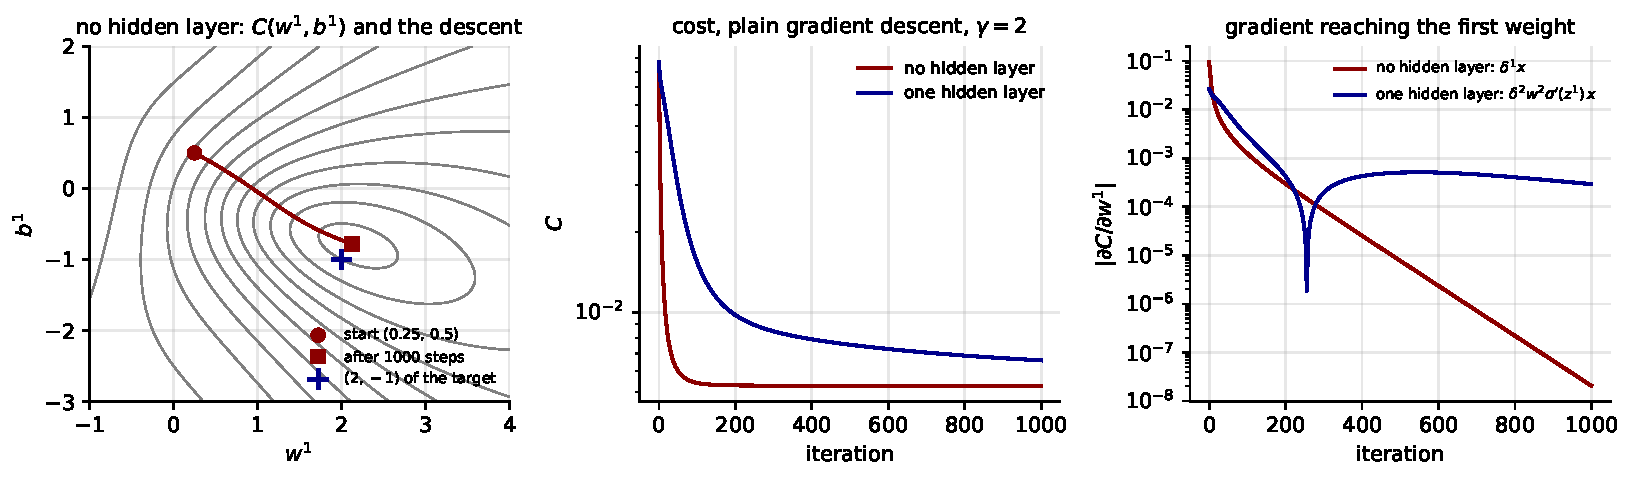
\includegraphics[width=0.98\textwidth]{BookFigures/chapter08_neural_networks/scalar_backprop}
\caption{The two scalar networks of Figure~\ref{fig:8-scalargraph} trained
by plain gradient descent, Eq.~(\ref{eq:8-scalarupdate}), on $n=20$ scalar
observations $y_i=\sigma(2x_i-1)+\varepsilon_i$ with $\gamma=2$ and $1000$
iterations, starting from $w^{1}=0.25$, $b^{1}=0.5$ (and $w^{2}=1$,
$b^{2}=-0.5$ for the hidden-layer network).  Left: the cost surface
$C(w^{1},b^{1})$ of the single neuron and the descent path from the starting
point (circle) to its end (square); the cross marks the parameters used to
generate the targets.  Middle: the cost against iteration for both networks.
Right: the magnitude of the gradient reaching the first weight, $\delta^{1}x$
in both cases, but with $\delta^{1}=\delta^{2}w^{2}\sigma'(z^{1})$ in the
deeper network, Eq.~(\ref{eq:8-scalardeltarec}); the extra factor
$w^{2}\sigma'(z^{2})$ attenuates the signal that trains the hidden neuron, a
first glimpse of Section~\ref{sec:vanishing}.  Generated by
\texttt{BookFigures/ch08\_scalar\_backprop\_figures.py}.}
\label{fig:8-scalartrain}
\end{figure}

\begin{notebox}
\textbf{What the general case adds.}  The two examples contain the whole
algorithm.  A layer with many nodes changes two things only.  A weight now
carries two node indices, $w_{ij}^{l}$, and the gradient
$\delta_j^{l}a_i^{l-1}$ pairs the error of the node it arrives at with the
activation of the node it leaves; and a hidden node feeds \emph{several}
nodes of the next layer, so the single term $\delta^{2}w^{2}$ of
Eq.~(\ref{eq:8-scalardeltarec}) becomes a sum $\sum_k\delta_k^{l+1}w_{jk}^{l+1}$
over everything it feeds -- the fan-out rule of Section~\ref{sec:adreverse},
exactly as the two branches of Figure~\ref{fig:5-logreggraph} were summed
when the reverse sweep reached $v_2$.  Section~\ref{sec:backpropgeneral} does
this bookkeeping, and Section~\ref{sec:backpropeqs} collects the result in
four equations that the reader may already recognise.
\end{notebox}

%......................................................................
\subsection{The general case: dense layers}
\label{sec:backpropgeneral}

Everything follows from the chain
